\subsection{Creating “Binless” Resampling Schemes: Na\textsuperscript{+}/Cl\textsuperscript{-} Association Simulations}

%%% For anyone trying to edit the source LaTeX code, the ~ are here to help space out the text so short words like 'Basic' doesn't get spread out across two lines. Sorry, there is no better solution. 

\subsubsection{Introduction}
The non-linearity of certain progress coordinates (e.g., those identified by machine learning tools) requires the creation of “binless” rather than binned resampling schemes for rare-event sampling. 
In addition, binless schemes can be useful in grouping trajectories by a feature of interest for resampling. 
For example,~ trajectories~ could~ be~ grouped~ by history~ (sharing the same parent structure) to improve the diversity of trajectories that successfully reach the target state, or by a simple k-means clustering. 
This tutorial builds upon the Basic WESTPA Tutorial (Na\textsuperscript{+}/Cl\textsuperscript{-} association simulations) \citep{bogetti_suite_2019} by introducing users to running and analyzing a WESTPA simulation that employs “binless” resampling schemes.
~ This~ tutorial~ is a prerequisite for \textbf{Advanced Tutorials 3.2-3.4}. 

\textbf{Learning Objectives.} This tutorial introduces users to the generalized resampler module in the WESTPA 2.0 software package that allows for the creation of either binned or binless resampling schemes.

The tutorial also instructs users on how to initiate a WE simulation from multiple representative conformations of the starting state and how to apply two key post-simulation analysis tools. 
Specific learning objectives are:
\begin{enumerate}
    \item How to create a binless scheme for splitting and merging trajectories based on k-means clustering using the \verb|BinlessMapper| resampler module;
    \item How to initiate a WE simulation from multiple starting conformations;
    \item How to combine multiple WE simulations for analysis using the \verb|w_multi_west| tool;
    \item How to perform post-simulation analysis using the \verb|w_crawl| tool.
\end{enumerate}

\subsubsection{Prerequisites}

\textbf{Computational Requirements.} This simulation can be completed in 5 hrs using 8 Intel Xeon W3550 3.07 GHz CPU cores, generating 1 GB of data using the HDF5 framework of the WESTPA 2.0 software package. 
Two independent \verb|west.h5| files, each containing 100 WE iterations of simulation data, are provided for the analysis portions of this tutorial in the \verb|for_analysis/| directory.
This tutorial uses the OpenMM 7.6 software package for dynamics propagation ({\url{https://openmm.org}}) and the MDTraj 1.9.5 analysis suite ({\url{https://www.mdtraj.org/1.9.5/index.html}}) for calculations of the WE progress coordinate. 
The scikit-learn 1.1.0 package ({\url{https://scikit-learn.org}}) is used to identify the “binless” groups.

\textbf{Jupyter Notebook.} Sample code for running and analyzing a WESTPA simulation according to “best practices” is made available in a Jupyter notebook.
For the visualization portions of the notebook, nglview, matplotlib, and ipympl are required. 

\textbf{Quick Start for this Tutorial.} Users can run the following command within the \verb|tutorial-3.1/| directory to install all the software dependencies for this tutorial to an existing conda environment:
\begin{verbatim}
  $ conda env update --name <your WESTPA conda env> 
                               --file environment.yml
\end{verbatim}

\subsubsection{Setting up the WE Simulation}
This simulation uses the same WE parameters ($\tau$, number of trajectories per bin, etc.) as the Basic WESTPA Tutorial (Na\textsuperscript{+}/Cl\textsuperscript{-} association simulations) \citep{bogetti_suite_2019}. 
The following are major differences from the Basic Tutorial that highlight more advanced features of WESTPA simulation setup.

\textbf{Binless Resampler Module.} The binless resampler module can be accessed from the \verb|west.cfg| file in the \verb|system_options| section where binned and binless schemes are all defined. 
If the \verb|BinlessMapper| is used by itself, the entirety of configurational space will be binless. 
To recycle trajectories while using a binless framework, we will need to place a \verb|BinlessMapper| inside of a \verb|RecursiveBinMapper| bin and demarcate the target state in a separate \verb|RecursiveBinMapper| bin. 
This framework is identical to the one used for the MAB scheme with recycling.

The \verb|BinlessMapper| takes three mandatory arguments. 
The first, \verb|ngroups|, specifies the total number of groups to assign trajectory walkers in the binless space. 
The second, \verb|ndims|, specifies the dimensionality of the progress coordinate and is limited to either 1 or 2 at this time. 
The \verb|ndims| parameter specifies the dimensionality of clustering, e.g., 2 for generating clusters in two-dimensional space (each dimension will not be grouped separately as is typically the case for binned resampling schemes). 
The clustering of trajectories enables sampling of high-dimensional space without an exponential increase in the number of walkers. 
The final argument is \verb|group_function|, which specifies the function for grouping trajectories in an external file (here, \verb|group.py|) and will take as input the progress coordinates and the \verb|ngroups| values. 
We provide a general example of using this function for a one-dimensional progress coordinate using k-means clustering. 
Additional keyword options can be specified under \verb|group_arguments| in the \verb|west.cfg| file. 
An example of using a recursive binless scheme is shown in the \verb|west.cfg| snippet below:

\begin{figure}[t]
\centering
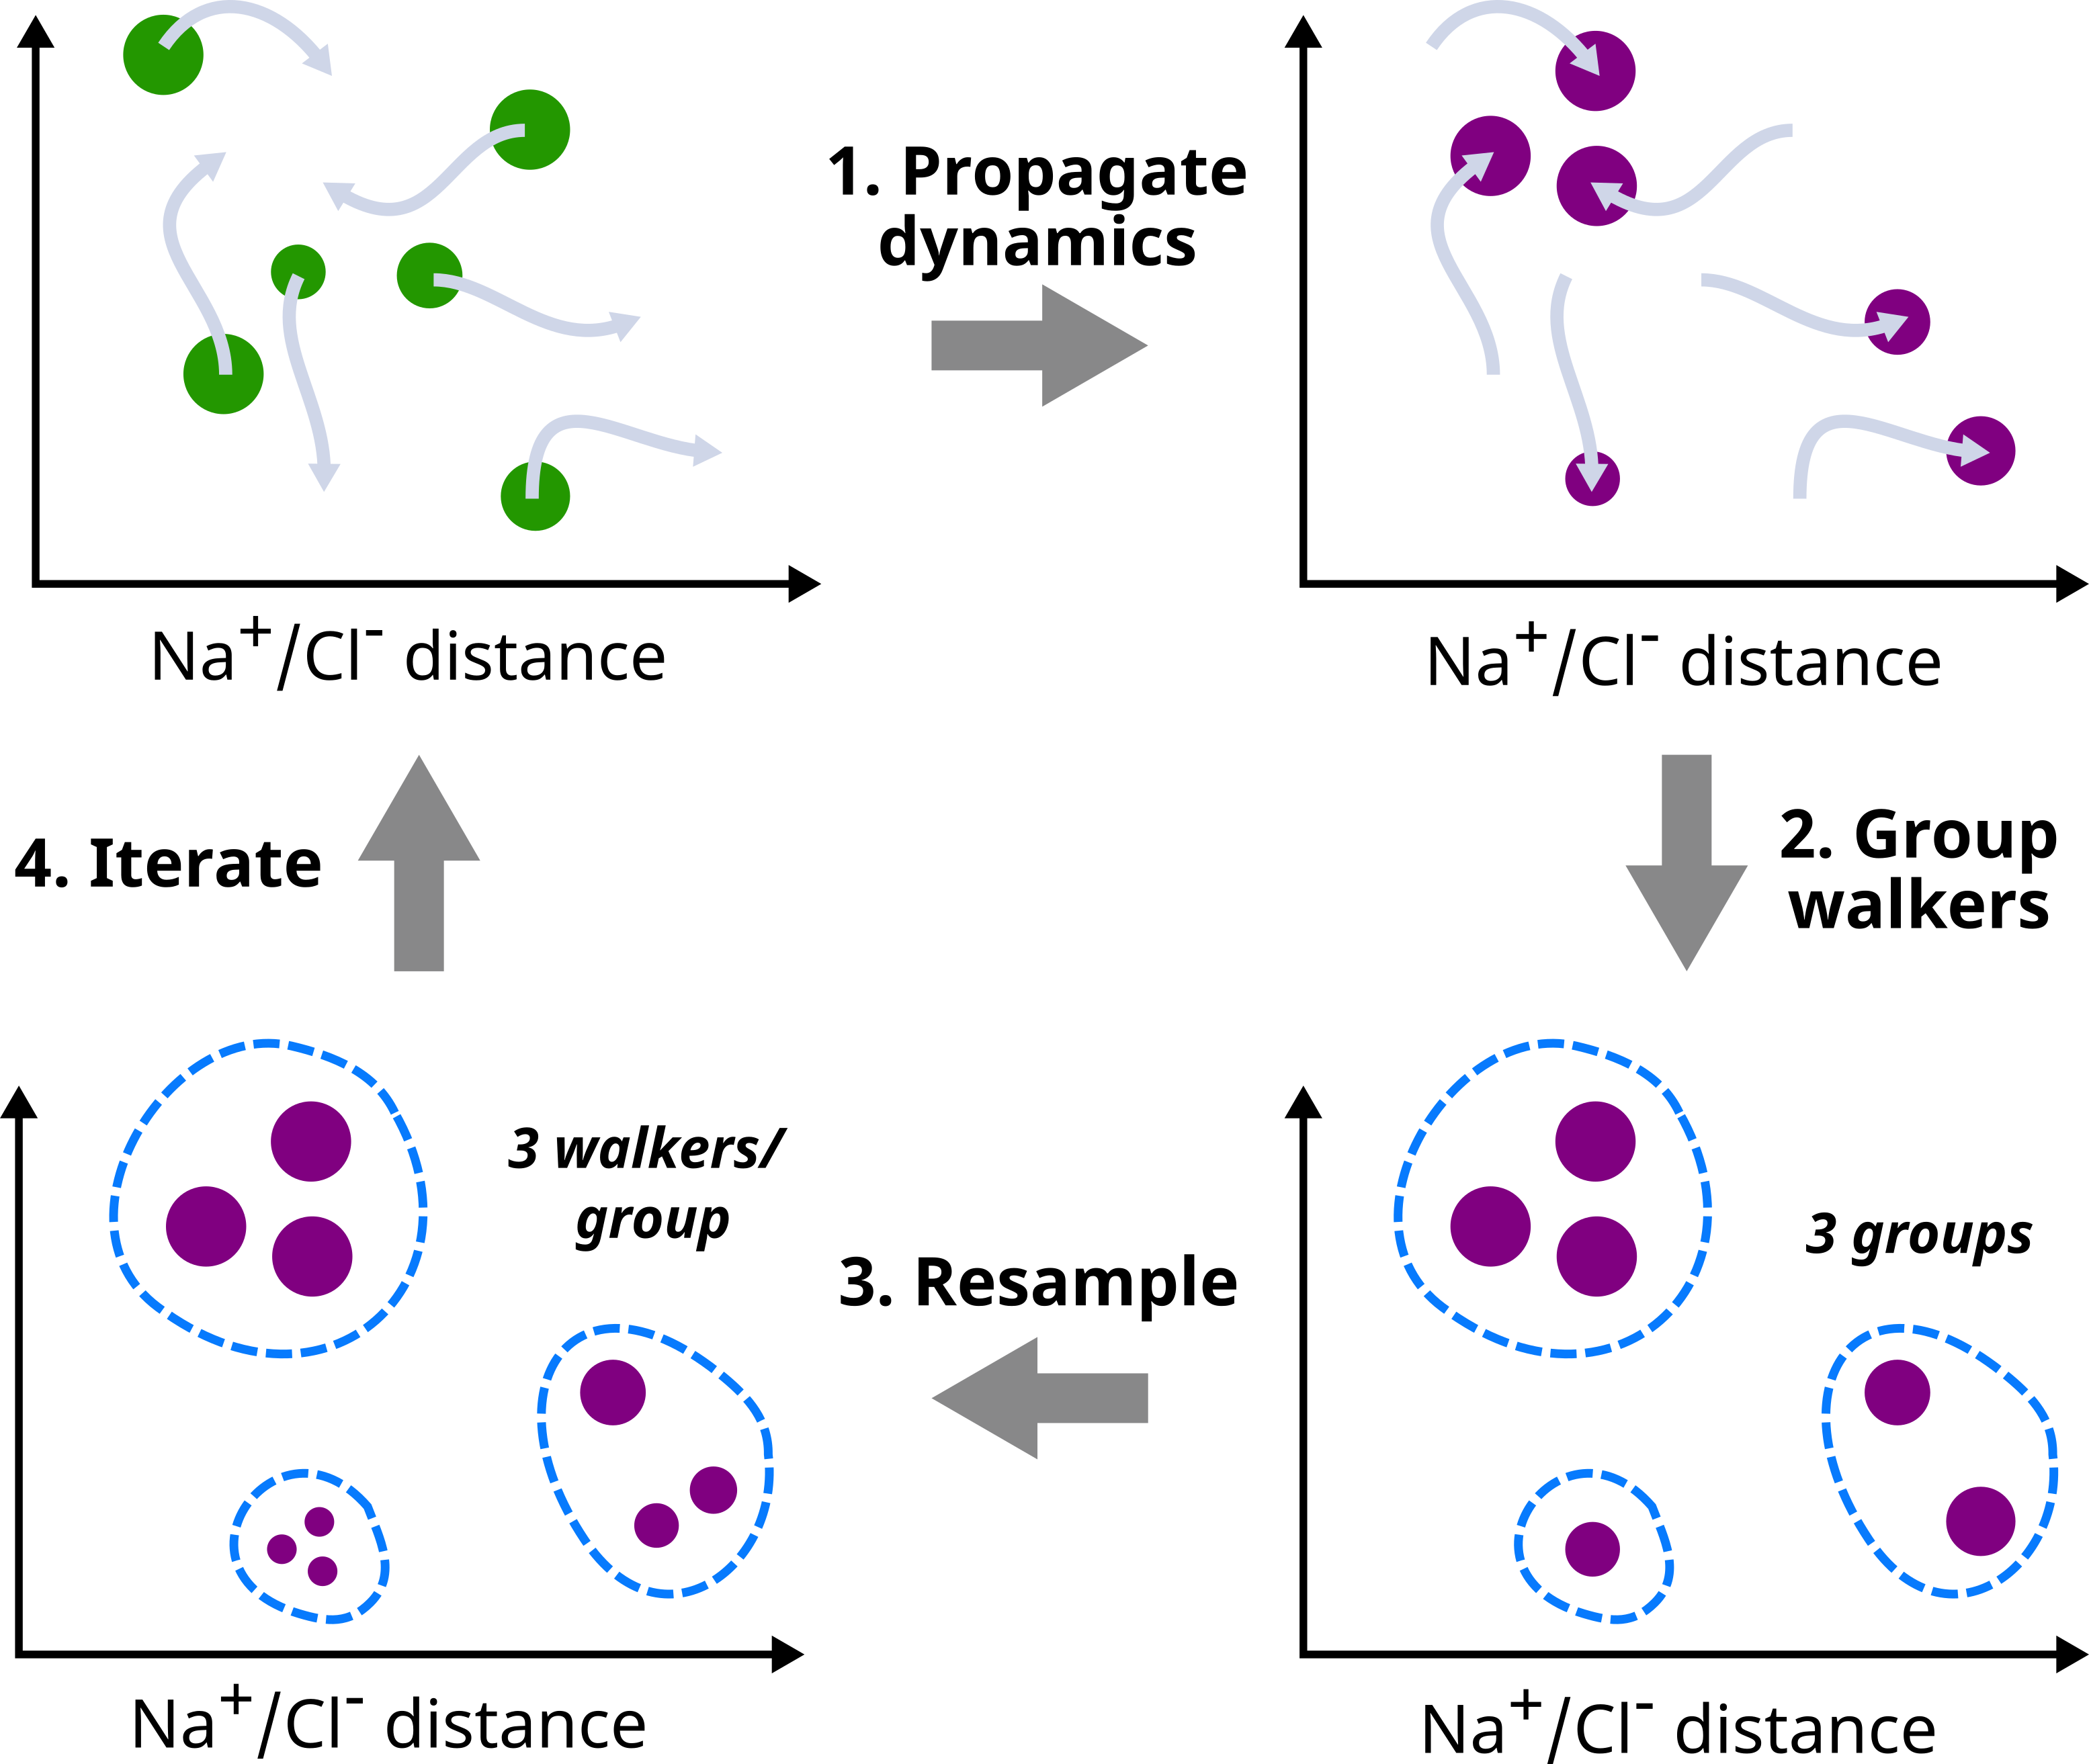
\includegraphics[width=\columnwidth]{figures/Figure3_binless.png}
\caption{Flow chart for simulating Na+/Cl- association using the new binless resampler module. 
After dynamics propagation in step 1, trajectories in each bin are grouped with the user-specified group.py function. 
In this example, trajectory walkers are grouped using k-means clustering.}
\end{figure}

\begin{verbatim}
  west:
    system:
      system_options:
        bins:
          type: RecursiveBinMapper
          base:
            type: RectilinearBinMapper
            boundaries:
              - [0, 2.60, 'inf']
            mappers:
            - type: BinlessMapper
              ngroups: [5] # Number of groups
              ndims: [1] # Number of grouping 
                         # dimensions
              group_function: group.kmeans
              at: [5]  # Location of binless mapper
                       # relative to base mapper
\end{verbatim} 

\textbf{Initiating a WE Simulation from Multiple Structures.} Ideally, a WE simulation is initiated from multiple pre-equilibrated structures that are representative of the initial state for the rare-event process of interest, e.g. using a conventional simulation or a separate WE simulation of the initial state.
Within the WESTPA framework, we refer to these structures as "basis states". 
If the simulation is run under non-equilibrium steady-state conditions, trajectories that reach the target state are “recycled” by terminating that trajectory and initiating a new trajectory with the same statistical weight from one of the basis states. 
Structural files (xml files in this tutorial) for basis states contain the coordinates and velocities, and are placed in separate, numbered folders within the \verb|bstates/| directory. 
Accompanying each xml file is a \verb|pcoord.init| text file which contains the progress coordinate value of that basis state. 
These progress coordinates are saved to the HDF5 file during the initialization process. 
The \verb|bstates/| directory also contains a reference file (\verb|bstates.txt|) that lists all of the available basis states. 
The \verb|bstates.txt| file is formatted with three columns, corresponding to the basis states’ names, associated probabilities, and folder name, respectively.
Additional basis states can be added as separate, additional lines at the end of the \verb|bstates.txt| file. 
The probability over all basis states must sum to one, and will be normalized by WESTPA during the initialization process to sum to one if the condition is not met.
Compared to the Basic WESTPA tutorial involving Na\textsuperscript{+}/Cl\textsuperscript{-} association \citep{bogetti_suite_2019}, the \verb|get_pcoord.sh| and \verb|runseg.sh| files are also modified such that \verb|$WEST_DATA_STRUCT_REF| now corresponds to the directory for each basis state and not the xml file itself.

\subsubsection{Running the WE Simulation}
As with previous versions of WESTPA, the simulation can be initialized using \verb|./init.sh| and run using \verb|./run.sh|. 
Alternatively, both steps could be executed consecutively using the new Python API by running the following command:

\begin{verbatim}
  $ python init_and_run.py
\end{verbatim}

The \verb|init_and_run.py| script will print out simulation updates to the console in real-time. 
An example \verb|runwe.slurm| file with commands for both methods of execution is provided for use with SLURM-like workload managers. 
We also provide a Jupyter notebook that demonstrates the steps for cleaning up, initializing, and running the WE simulation.

Note that this tutorial is using the new HDF5 trajectory storage framework, which will be explained further in \textbf{Advanced Tutorial 3.2}. 
To enable the use of the HDF5 framework in your own simulation, you may use the current tutorials directory as an example. 
The location of the trajectory h5 files will need to be specified in the \verb|west.cfg| file, and the appropriate restart and topology files will need to be copied to the locations specified in the \verb|get_pcoord.sh| and \verb|runseg.sh| files. 
You will also need to make sure that the file extensions for any trajectory files are readable by \verb|mdtraj.load|, (e.g., Amber restart files must end in .ncrst) which simply requires renaming. 
To save disk space, trajectory files outputted by the dynamics engine can be deleted after every iteration in the \verb|post_iter.sh| file, which is located in the \verb|westpa_scripts/| directory.

\subsubsection{Monitoring and Analyzing the WE Simulation}

\textbf{Combining Multiple WE Simulations for Analysis.} To combine multiple WE simulations into a single aggregate simulation file for analysis, we can use the \verb|w_multi_west| tool, which creates a single \verb|multi.h5| file that contains the data from all of the \verb|west.h5| files of each WE simulation. 
Each WE iteration in the \verb|multi.h5| file contains all of the trajectory segments from the corresponding iterations of the individual WE simulations, all normalized to the total weight for that iteration. 
For backwards compatibility, a version of \verb|w_multi_west| for use with previously run WESTPA 1.0 simulations (v2020.XX) has been available since version 2020.04.

To apply the multitool to a combination of \verb|west.h5| files, place the \verb|west.h5| file for each simulation in a numbered directory starting with \verb|01/|. 
If all of the simulations used a custom grouping function (such as in \verb|group.py|), you must also include that file in the top-level analysis directory. 

The files will be organized as follows:
\begin{verbatim}
  01/
    west.h5
  02/
    west.h5
  group.py [if used in simulation]
\end{verbatim}

Next, in this directory, run the following to merge the \verb|west.h5| files:
\begin{verbatim}
  $ w_multi_west -m . -n 2
\end{verbatim}

The \verb|-m| flag specifies the path to your directories and the \verb|-n| flag specifies the number of WE simulations to combine for analysis. 
To combine auxiliary datasets, one can add either an \verb|--aux=NAME_OF_DATASET| flag for a specific dataset or an \verb|--auxall| flag for all auxiliary datasets; note that the inclusion of auxiliary datasets will substantially extend the time needed to combine the simulation data. 
The above \verb|w_multi_west --auxall| command will generate a list of WE simulation datasets to combine based on the datasets listed in \verb|01/west.h5| and generate a \verb|multi.h5| file with the combined simulation datasets. 
You may want to rename this file to \verb|west.h5| in order to apply the \verb|w_pdist| tool to the combined simulation dataset. 
Note that the \verb|w_multi_west| tool will only merge up to the \textit{N-1} WE iteration, ignoring the last WE iteration. 
The resulting \verb|multi.h5| file will not link to the individual iteration HDF5 files generated using the HDF5 framework.

\textbf{Post-Simulation Analysis.} As mentioned above, WESTPA 2.0 enables efficient post-simulation analysis of trajectory data by storing trajectory data in highly compressed HDF5 files. 
The \verb|w_crawl| tool can then be used to “crawl” through the trajectory data in single HDF5 files per WE iteration rather than millions of trajectory files.
Results from the analysis are written to a dataset in a new HDF5 file. 
Before crawling through an entire simulation dataset, we recommend that users first test their analysis scheme in the \verb|wcrawl_functions.py| file to ensure that the scheme works as expected. 
For this tutorial, we will only be using a single CPU core for these \verb|w_crawl| calculations but also include a sample script as an example of how to use \verb|w_crawl| on multiple CPU cores in parallel. 
The \verb|wcrawl_functions.py| file contains the main analysis code. 
This script first identifies the final frame of a segment’s parent trajectory file from the previous WE iteration and makes sure this is eventually combined with the trajectory segment from the current WE iteration. 
The inclusion of the parent structure at the beginning of the current iteration trajectory is necessary for using the crawled dataset with WESTPA’s kinetics analysis tools. 
In this example, trajectory coordinates of only Na\textsuperscript{+} and Cl\textsuperscript{-} are extracted using the MDTraj analysis suite and multiplied by 10 to convert from nm to \AA. 
Resulting per-iteration coordinate values are then saved to an array, which is subsequently saved to a \verb|coord.h5| file. 
The \verb|coord.h5| file is formatted similarly to a \verb|west.h5| file, where the new per-iteration values are stored under \verb|iterations/iter_{n_iter:08d}/coord|. 
To ease analysis, a \verb|copy_h5_dataset.py| script is provided to copy \verb|coord.h5|’s contents into a west.h5 file as an auxiliary dataset. 
Note that if you store a WESTPA simulation's trajectory HDF5 files in a separate directory from what is used in this tutorial, you need to specify the directory where the \verb|iter_XXXXXX.h5| files are located in the \verb|wcrawl_functions.py| file.

The \verb|run_w_crawl.sh| shell script runs the \verb|w_crawl| tool at the command line and provides options for running the tool in serial or parallel modes. 
In this tutorial example, we will run the \verb|w_crawl| tool in the serial mode using the \verb|--serial| flag, analyzing one WE iteration at a time on a single CPU core. 
While the serial mode is sufficient for “crawling” relatively small datasets, the parallel mode using the \verb|--parallel| flag is desirable for datasets with over 100 trajectory segments per WE iteration and/or hundreds of WE iterations. 
In the parallel mode, each CPU core of a single compute node analyzes a different WE iteration at the same time. 
To run the \verb|w_crawl| tool across multiple nodes, one can use the ZMQ work manager.
Once satisfied with the \verb|wcrawl_functions.py| and \verb|run_w_crawl.sh| files, run the \verb|w_crawl| tool locally:

\begin{verbatim}
  $ ./run_w_crawl.sh
\end{verbatim}

or on a multi-node cluster using the Slurm workload manager:

\begin{verbatim}
  $ sbatch run_w_crawl.sh
\end{verbatim}

To monitor the progress of the analysis, we examine the \verb|w_crawl.log| file, which contains analysis results for each WE iteration and each trajectory segment.
Finally, to copy the \verb|coord.h5| file to the \verb|west.h5| file, run the \verb|copy_h5_dataset.py| script.

\subsubsection{Conclusion} After completing this tutorial, users will gain an understanding of how to configure the upgraded resampler module for using a binless scheme, initiate a WE simulation from multiple structures using the new HDF5 trajectory storage framework, and apply the \verb|w_multi_west| and \verb|w_crawl| post-simulation analysis tools. 